%%%%%%%%%%%%%%%%%%%%%%%%%%%%%%%%%%%%%%%%%
% Beamer Presentation
% LaTeX Template
% Version 1.0 (10/11/12)
%
% This template has been downloaded from:
% http://www.LaTeXTemplates.com
%
% License:
% CC BY-NC-SA 3.0 (http://creativecommons.org/licenses/by-nc-sa/3.0/)
%
%%%%%%%%%%%%%%%%%%%%%%%%%%%%%%%%%%%%%%%%%

%----------------------------------------------------------------------------------------
%	PACKAGES AND THEMES
%----------------------------------------------------------------------------------------
\documentclass{beamer}
\usepackage{tikz}
\usetikzlibrary{shapes,arrows,shadows}
\usetikzlibrary{automata,positioning,arrows}
\usepackage{amsmath,bm,times}
\usetikzlibrary{backgrounds}

\mode<presentation> {

% The Beamer class comes with a number of default slide themes
% which change the colors and layouts of slides. Below this is a list
% of all the themes, uncomment each in turn to see what they look like.

%\usetheme{default}
%\usetheme{AnnArbor}
%\usetheme{Antibes}
%\usetheme{Bergen}
\usetheme{Berkeley}
%\usetheme{Berlin}
%\usetheme{Boadilla}
%\usetheme{CambridgeUS}
%\usetheme{Copenhagen}
%\usetheme{Darmstadt}
%\usetheme{Dresden}
%\usetheme{Frankfurt}
%\usetheme{Goettingen}
%\usetheme{Hannover}
%\usetheme{Ilmenau}
%\usetheme{JuanLesPins}
%\usetheme{Luebeck}
%\usetheme{Madrid}
%\usetheme{Malmoe}
%\usetheme{Marburg}
%\usetheme{Montpellier}
%\usetheme{PaloAlto}
%\usetheme{Pittsburgh}
%\usetheme{Rochester}
%\usetheme{Singapore}
%\usetheme{Szeged}
%\usetheme{Warsaw}

% As well as themes, the Beamer class has a number of color themes
% for any slide theme. Uncomment each of these in turn to see how it
% changes the colors of your current slide theme.

%\usecolortheme{albatross}
%\usecolortheme{beaver}
%\usecolortheme{beetle}
%\usecolortheme{crane}
%\usecolortheme{dolphin}
%\usecolortheme{dove}
%\usecolortheme{fly}
%\usecolortheme{lily}
%\usecolortheme{orchid}
%\usecolortheme{rose}
%\usecolortheme{seagull}
\usecolortheme{seahorse}
%\usecolortheme{whale}
%\usecolortheme{wolverine}

%\setbeamertemplate{footline} % To remove the footer line in all slides uncomment this line
%\setbeamertemplate{footline}[page number] % To replace the footer line in all slides with a simple slide count uncomment this line

%\setbeamertemplate{navigation symbols}{} % To remove the navigation symbols from the bottom of all slides uncomment this line
}

\usepackage{graphicx} % Allows including images
\usepackage{booktabs} % Allows the use of \toprule, \midrule and \bottomrule in tables
\setbeamertemplate{navigation symbols}{}
%----------------------------------------------------------------------------------------
%	TITLE PAGE
%----------------------------------------------------------------------------------------

\title[\textsc{Scaffolding}]{\textsc{Evaluation and benchmarking of a new scaffolding methodology}} % The short title appears at the bottom of every slide, the full title is only on the title page

\author{\textsc{Alexandrina Bodrug}} % Your name
\institute[\textsc{genscale, irisa}] % Your institution as it will appear on the bottom of every slide, may be shorthand to save space
{
\textit{\textsc{\tiny Supervisors: Pr. Rumen Andonov \& Dr. Dominique Lavenier}} \\
\vspace*{1cm}
\textsc{University Rennes 1} \\ % Your institution for the title page
\textit{\textsc{\tiny Bioinformatics and Genomics Master}} % Your email address
}
\date{\tiny \textsc{June 25, 2015}} % Date, can be changed to a custom date

\begin{document}

\begin{frame}
\titlepage % Print the title page as the first slide
\end{frame}

\begin{frame}
\frametitle{Overview} % Table of contents slide, comment this block out to remove it
\tableofcontents % Throughout your presentation, if you choose to use \section{} and \subsection{} commands, these will automatically be printed on this slide as an overview of your presentation
\end{frame}

%----------------------------------------------------------------------------------------
%	PRESENTATION SLIDES
%----------------------------------------------------------------------------------------

%------------------------------------------------
\section{Context}\label{context}
\begin{frame}
\frametitle{\textsc{\nameref{context}}}
\resizebox{10.5cm}{!}{
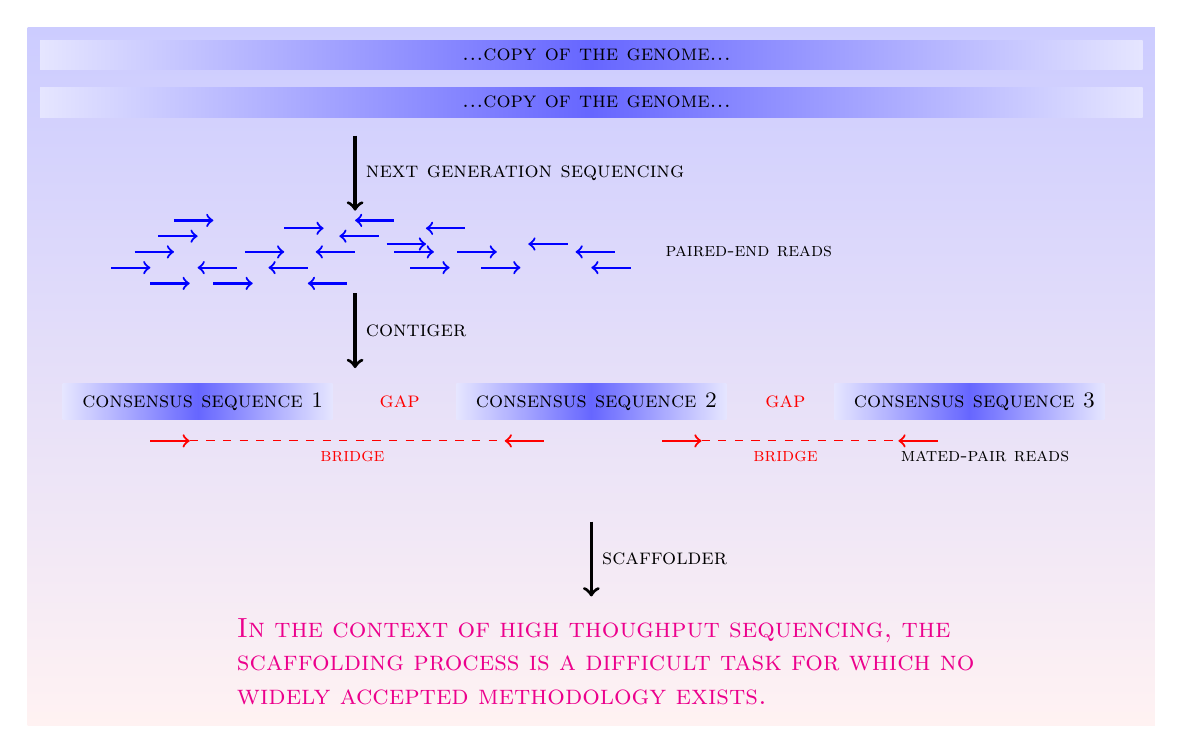
\begin{tikzpicture}[framed,background rectangle/.style={top color=blue!20, bottom color=pink!20}]
    \node[left color=blue!10, right color=blue!10, middle color=blue!60, minimum width = 14cm](copy1) at (3,0) {\textsc{ \footnotesize ...copy of the genome...}};
    \draw[draw=none](copy1.north west)--(copy1.north east) (copy1.south west)--(copy1.south east);
    \node[left color=blue!10, right color=blue!10, middle color=blue!60, minimum width = 14cm](copy2) at (3,0.6) {\textsc{ \footnotesize ...copy of the genome...}};
    \draw[draw=none](copy2.north west)--(copy2.north east) (copy2.south west)--(copy2.south east);
    
    \node (a) at (0,-0.3) {};
    \node (b) at (0,-1.5) {};
    \draw[very thick, ->] (a.south) -- node[right] {\footnotesize \textsc{next generation sequencing}}  (b.north);

\node[] (pe) at (5,-1.9) {\scriptsize \textsc{paired-end reads}};
\node[] (mp) at (8,-4.5) {\scriptsize \textsc{mated-pair reads}};

\begin{scope}[shift={(-3,0)}]
\draw[blue, thick, <-] (3,-1.5) -- (3.5,-1.5);
%\draw[blue, dashed] (3,-1.5) -- (1.2,-1.5);
\draw[blue, thick, ->] (0.7,-1.5) -- (1.2,-1.5);
\end{scope}
\begin{scope}[shift={(-3.2,-0.2)}]
\draw[blue, thick, <-] (3,-1.5) -- (3.5,-1.5);
%\draw[blue, dashed] (3,-1.5) -- (1.2,-1.5);
\draw[blue, thick, ->] (0.7,-1.5) -- (1.2,-1.5);
\end{scope}
\begin{scope}[shift={(-3.5,-0.4)}]
\draw[blue, thick, <-] (3,-1.5) -- (3.5,-1.5);
%\draw[blue, dashed] (3,-1.5) -- (1.2,-1.5);
\draw[blue, thick, ->] (0.7,-1.5) -- (1.2,-1.5);
\end{scope}
\begin{scope}[shift={(0,-0.6)}]
\draw[blue, thick, <-] (3,-1.5) -- (3.5,-1.5);
%\draw[blue, dashed] (3,-1.5) -- (1.2,-1.5);
\draw[blue, thick, ->] (0.7,-1.5) -- (1.2,-1.5);
\end{scope}
\begin{scope}[shift={(-0.2,-0.4)}]
\draw[blue, thick, <-] (3,-1.5) -- (3.5,-1.5);
%\draw[blue, dashed] (3,-1.5) -- (1.2,-1.5);
\draw[blue, thick, ->] (0.7,-1.5) -- (1.2,-1.5);
\end{scope}
\begin{scope}[shift={(-0.8,-0.3)}]
\draw[blue, thick, <-] (3,-1.5) -- (3.5,-1.5);
%\draw[blue, dashed] (3,-1.5) -- (1.7,-1.5);
\draw[blue, thick, ->] (1.2,-1.5) -- (1.7,-1.5);
\end{scope}
\begin{scope}[shift={(-1.1,-0.1)}]
\draw[blue, thick, <-] (2,-1.5) -- (2.5,-1.5);
%\draw[blue, dashed] (2,-1.5) -- (0.7,-1.5);
\draw[blue, thick, ->] (0.2,-1.5) -- (0.7,-1.5);
\end{scope}
\begin{scope}[shift={(-1.1,-0.1)}]
\draw[blue, thick, <-] (0,-2) -- (0.5,-2);
%\draw[blue, dashed] (2,-2) -- (0.7,-2);
\draw[blue, thick, ->] (-2,-2) -- (-1.5,-2);
\end{scope}
\begin{scope}[shift={(-1.1,-0.1)}]
\draw[blue, thick, <-] (0.5,-2.2) -- (1,-2.2);
%\draw[blue, dashed] (2,-2) -- (0.7,-2);
\draw[blue, thick, ->] (-1.5,-2.2) -- (-1,-2.2);
\draw[blue, thick, ->] (-0.7,-2.2) -- (-0.2,-2.2);
\draw[blue, thick, <-] (-0.9,-2) -- (-0.4,-2);
\draw[blue, thick, ->] (-0.3,-1.8) -- (0.2,-1.8);
\draw[blue, thick, ->] (2.4,-1.8) -- (2.9,-1.8);
\draw[blue, thick, ->] (2.7,-2) -- (3.2,-2);
\end{scope}

    \node (c) at (0,-2.3) {};
    \node (d) at (0,-3.5) {};
    \draw[very thick, ->] (c.south) -- node[right] {\footnotesize \textsc{contiger}}  (d.north);
    
\node[left color=blue!10, right color=blue!10, middle color=blue!60](cs1) at (-2,-3.8) {\textsc{ \footnotesize consensus sequence 1}};
\node[left color=blue!10, right color=blue!10, middle color=blue!60](cs2) at (3,-3.8) {\textsc{ \footnotesize consensus sequence 2}};
\node[left color=blue!10, right color=blue!10, middle color=blue!60](cs3) at (7.8,-3.8) {\textsc{ \footnotesize consensus sequence 3}};
\node[red](gap1) at (0.5,-3.8) {\textsc{ \footnotesize gap}};
\node[red](gap2) at (5.4,-3.8) {\textsc{ \footnotesize gap}};

\begin{scope}[shift={(-1.1,-2.5)}]
\draw[red, thick, <-] (3,-1.8) -- (3.5,-1.8);
\draw[red, dashed] (-1,-1.8) -- (3,-1.8);
\draw[red, thick, ->] (-1.5,-1.8) -- (-1,-1.8);
\node[red](gap2) at (1,-2) {\textsc{ \scriptsize bridge}};

\draw[red, thick, <-] (8,-1.8) -- (8.5,-1.8);
\draw[red, dashed] (5.5,-1.8) -- (8,-1.8);
\draw[red, thick, ->] (5,-1.8) -- (5.5,-1.8);
\node[red](gap2) at (6.5,-2) {\textsc{ \scriptsize bridge}};

\end{scope}


    \node (e) at (3,-5.2) {};
    \node (f) at (3,-6.4) {};
    \draw[very thick, ->] (e.south) -- node[right] {\footnotesize \textsc{scaffolder}}  (f.north);

\node[text width = 10cm] (scaf) at (3.5, -7.1) {\textsc{\textcolor{magenta}{In the context of high thoughput sequencing, the scaffolding process is a difficult task for which no widely accepted methodology exists.}}};


\end{tikzpicture}
}
\end{frame}
\subsection{Some definitions}\label{defs}
\begin{frame}
\frametitle{\textsc{\nameref{defs}}}
\texttt{"The \textit{Contig Scaffolding Problem}  is to order and orientate the given \textcolor{magenta}{contigs} in a manner that is consistent with as many mate-pairs as possible".}
\begin{center}
Hudson \textit{et al.} 2002
\end{center}
\end{frame}

\begin{frame}
\frametitle{\textsc{\nameref{defs}}}
\footnotesize Genome is fragmented, extremities are sequenced ($\mapsto$ reads) \ldots \\
\resizebox{7cm}{!}{
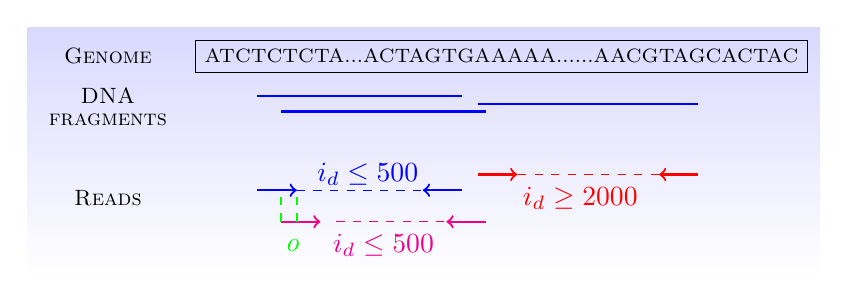
\begin{tikzpicture}[framed,background rectangle/.style={top color=blue!15}]
\node[draw=none] at (-4,0) {\footnotesize \textsc{Genome}};
\node[draw] at (1,0) {\scriptsize ATCTCTCTA...ACTAGTGAAAAA......AACGTAGCACTAC};
\node[draw=none] at (-4,-0.5) {\footnotesize \textsc{DNA}};
\node[draw=none] at (-4,-0.8) {\footnotesize \textsc{fragments}};
\draw[thick, blue] (-2.1, -0.5) -- (0.5, -0.5);
\draw[thick, blue] (0.7, -0.6) -- (3.5, -0.6);
\draw[thick, blue] (-1.8, -0.7) -- (0.8, -0.7);
\node[draw=none] at (-4,-1.8) {\footnotesize \textsc{Reads}};

\draw[red, thick, <-] (3,-1.5) -- (3.5,-1.5);
\draw[red, dashed] (3,-1.5) -- (1.2,-1.5);
\node[draw=none, color=red] at (2,-1.8) {\textit{$i_d \geq 2000$}};
\draw[red, thick, ->] (0.7,-1.5) -- (1.2,-1.5);

\draw[blue, thick, <-] (0,-1.7) -- (0.5,-1.7);
\draw[blue, dashed] (-1.6,-1.7) -- (0,-1.7);
\node[draw=none, color=blue] at (-0.7,-1.5) {\textit{$i_d\leq 500$}};
\draw[blue, thick, ->] (-2.1,-1.7) -- (-1.6,-1.7);

\draw[magenta, thick, <-] (0.3,-2.1) -- (0.8,-2.1);
\draw[magenta, dashed] (-1.1,-2.1) -- (0.3,-2.1);
\node[draw=none, color=magenta] at (-0.5,-2.4) {\textit{$i_d\leq 500$}};
\draw[magenta, thick, ->] (-1.8,-2.1) -- (-1.3,-2.1);

\node[draw=none, color=green] at (-1.65, -2.4) {\textit{o}};
\draw[green, dashed, thick] (-1.8, -2.1) -- (-1.8, -1.7); 
\draw[green, dashed, thick] (-1.6, -2.1) -- (-1.6, -1.7);
\end{tikzpicture}
}\\
\footnotesize \ldots reads are assembled into consensus sequences. \\ \textsc{\textcolor{magenta}{Unitigs are high confidence contigs.}} \\
\vspace*{0.2cm}
\resizebox{8cm}{!}{
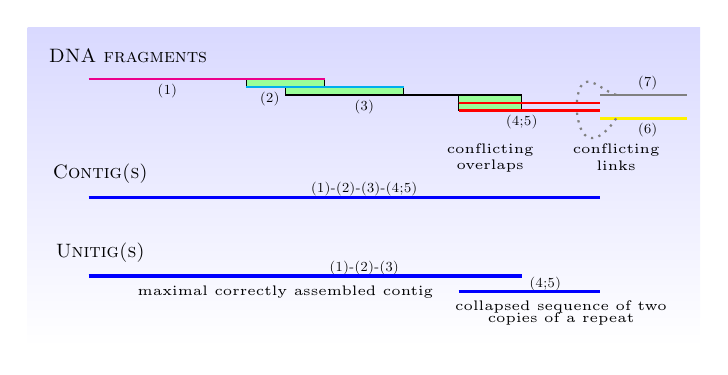
\begin{tikzpicture}[framed,background rectangle/.style={ top color=blue!15}]
\node[draw=none] at (1,0.3) {\scriptsize \textsc{DNA fragments}};
\node[draw=none] at (1.5,-0.15) {\tiny \textsc{(1)}};
\node[draw=none] at (2.8,-0.25) {\tiny \textsc{(2)}};
\node[draw=none] at (4,-0.35) {\tiny \textsc{(3)}};
\node[draw=none] at (6,-0.55) {\tiny \textsc{(4;5)}};
\node[draw=none] at (7.6,-0.65) {\tiny \textsc{(6)}};
\node[draw=none] at (7.6,-0.05) {\tiny \textsc{(7)}};
\node[draw=none] at (4,-1.4) {\tiny \textsc{(1)-(2)-(3)-(4;5)}};
\node[draw=none] at (4,-2.4) {\tiny \textsc{(1)-(2)-(3)}};
\node[draw=none] at (6.3,-2.6) {\tiny \textsc{(4;5)}};

\draw[fill=green!40] (2.5,0) -- (3.5,0) -- (3.5,-0.1) -- (2.5,-0.1) -- (2.5,0);
\draw[fill=green!40] (3,-0.1) -- (4.5,-0.1) -- (4.5,-0.2) -- (3,-0.2) -- (3,-0.1);
\draw[fill=green!40] (5.2,-0.2) -- (6.0,-0.2) -- (6.0,-0.3) -- (5.2,-0.3) -- (5.2,-0.2);
\draw[fill=green!40] (5.2,-0.3) -- (6.0,-0.3) -- (6.0,-0.4) -- (5.2,-0.4) -- (5.2,-0.3);

\draw[thick, magenta] (0.5,0) -- (3.5,0);
\draw[thick, cyan] (2.5,-0.1) -- (4.5,-0.1);
\draw[thick, black] (3.0,-0.2) -- (6.0,-0.2);
\draw[thick, red] (5.2,-0.3) -- (7,-0.3);
\draw[thick, red] (5.2,-0.4) -- (7,-0.4);
\draw[thick, yellow!] (7.0,-0.5) -- (8.1,-0.5);
\draw[thick, gray] (7.0,-0.2) -- (8.1,-0.2);

\draw[color=gray, dotted, thick] (7.2,-0.2) .. controls  (7,-0.15) and (6.75,0.2) .. (6.7,-0.3);
\draw[color=gray, dotted, thick] (7.2,-0.5) .. controls  (7,-0.8) and (6.75,-0.9) .. (6.7,-0.4);

\node[draw=none] at (5.6,-0.9) {\tiny conflicting};
\node[draw=none] at (5.6,-1.1) {\tiny overlaps};
\node[draw=none] at (7.2,-0.9) {\tiny conflicting};
\node[draw=none] at (7.2,-1.1) {\tiny links};
\node[draw=none] at (0.65,-1.2) {\scriptsize \textsc{Contig(s)}};
\draw[very thick, blue] (0.5, -1.5) -- (7, -1.5);
\node[draw=none] at (0.65,-2.2) {\scriptsize \textsc{Unitig(s)}};
\draw[very thick, blue] (0.5, -2.5) -- (6.0, -2.5);
\node[draw=none] at (3,-2.7) {\tiny maximal correctly assembled contig};
\draw[very thick, blue] (5.2, -2.7) -- (7, -2.7);
\node[draw=none] at (6.5,-2.9) {\tiny collapsed sequence of two };
\node[draw=none] at (6.5,-3.05) {\tiny copies of a repeat};
\end{tikzpicture}
}


\end{frame}
\subsection{Order and orient}\label{oando}
\begin{frame}
\frametitle{\textsc{\nameref{oando}}}
\begin{center}
Mated-pair read $\mapsto$ bridge between contigs\\
Several correctly mapped reads $\mapsto$ link between contigs  \\
High-confidence overlap $\mapsto$ link between contigs \\
All linkage information $\mapsto$ order and orient contigs \\
\vspace*{1cm}
\textsc{\textcolor{magenta}{Conflicting links can and will exist.}}
\end{center}

\end{frame}

\subsection{Challenging problem}\label{challenge}
\begin{frame}
\frametitle{\textsc{\nameref{challenge}}}
What would you do in these situations?
\resizebox{4in}{!}{
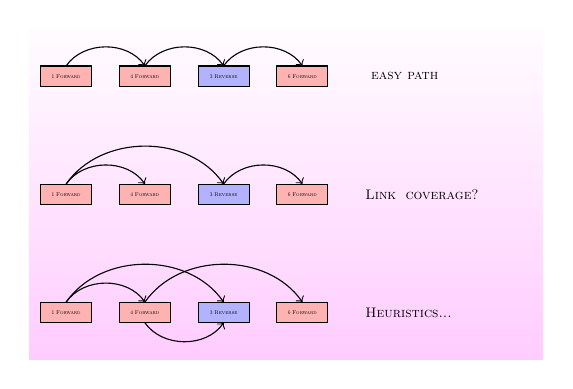
\begin{tikzpicture}[framed,background rectangle/.style={draw=white, bottom color=magenta!20, top color=magenta!1}]
\node (1F) [draw, text width=3cm, minimum height=1.3cm, fill=red!30, scale=0.2, align=center] at (0,0) {1 \textsc{Forward}};
\node (4F) [draw, text width=3cm, minimum height=1.3cm, fill=red!30, scale=0.2, align=center] at (1,0) {4 \textsc{Forward}};
\node (3R) [draw, text width=3cm, minimum height=1.3cm, fill=blue!30, scale=0.2, align=center] at (2,0) {3 \textsc{Reverse}};
\node (6F) [draw, text width=3cm, minimum height=1.3cm, fill=red!30, scale=0.2, align=center] at (3,0) {6 \textsc{Forward }};
\draw[->] (1F.north) to [bend left=55] (4F.north);
\draw[->] (4F.north) to [bend left=55] (3R.north);
\draw[->] (3R.north) to [bend left=55] (6F.north);

\begin{scope}[yshift=-1.5cm]
\node (1F) [draw, text width=3cm, minimum height=1.3cm, fill=red!30, scale=0.2, align=center] at (0,0) {1 \textsc{Forward}};
\node (4F) [draw, text width=3cm, minimum height=1.3cm, fill=red!30, scale=0.2, align=center] at (1,0) {4 \textsc{Forward}};
\node (3R) [draw, text width=3cm, minimum height=1.3cm, fill=blue!30, scale=0.2, align=center] at (2,0) {3 \textsc{Reverse}};
\node (6F) [draw, text width=3cm, minimum height=1.3cm, fill=red!30, scale=0.2, align=center] at (3,0) {6 \textsc{Forward }};
\draw[->] (1F.north) to [bend left=55] (4F.north);
\draw[->] (1F.north) to [bend left=55] (3R.north);
%\draw[->] (4F.north) to [bend left=55] (3R.north);
\draw[->] (3R.north) to [bend left=55] (6F.north);
\end{scope}
\begin{scope}[yshift=-3cm]
\node (1F) [draw, text width=3cm, minimum height=1.3cm, fill=red!30, scale=0.2, align=center] at (0,0) {1 \textsc{Forward}};
\node (4F) [draw, text width=3cm, minimum height=1.3cm, fill=red!30, scale=0.2, align=center] at (1,0) {4 \textsc{Forward}};
\node (3R) [draw, text width=3cm, minimum height=1.3cm, fill=blue!30, scale=0.2, align=center] at (2,0) {3 \textsc{Reverse}};
\node (6F) [draw, text width=3cm, minimum height=1.3cm, fill=red!30, scale=0.2, align=center] at (3,0) {6 \textsc{Forward }};
\draw[->] (1F.north) to [bend left=55] (4F.north);
\draw[->] (1F.north) to [bend left=55] (3R.north);
\draw[->] (4F.north) to [bend left=55] (6F.north);
\draw[->] (4F.south) to [bend left=-55] (3R.south);
\end{scope}

\begin{scope}[xshift=4.3cm]
\node[] at (0,0) {\textsc{\tiny easy path}};
\node[text width =2cm] at (0.5,-1.5) {\textsc{\tiny Link coverage?}};
\node[text width =2cm] at (0.5,-3) {\textsc{\tiny Heuristics...}};
\end{scope}
\end{tikzpicture}
}
\end{frame}

\section{GST features}\label{GST}
\begin{frame}
\frametitle{\textsc{Genscale scaffolding tools features}}

\textsc{\textcolor{magenta}{Several tools model the problem differently.}}
\vspace*{0.5cm} \\
\footnotesize
$\to$ common features: 
\begin{itemize}
\item modeling of the scaffolding problem as a \textcolor{magenta}{graph}
\item use of unitigs instead of contigs to better compute coverage
\item use of \textcolor{magenta}{unitig coverages to duplicate nodes} representing unitigs
\item unitig orientations represented by separate nodes
\end{itemize}
$\to$ differences: 
\begin{itemize}
\item \textbf{weighted path model} focuses solely on order and orientation
\item \textbf{distance based model} incorporates \textcolor{magenta}{link length} information
\item \textbf{flow model} accepts \textcolor{magenta}{intervals} for unitig coverage and link length
\end{itemize}
\end{frame}

\subsection{Scripting for the GST}\label{scripting}
\begin{frame}
\frametitle{\textsc{Handling the modeled graphs}}
Automated ways to control the input data and validate the scaffolding solution:
\begin{itemize}
\item a script to visualize input data and GST solutions: \texttt{graph\_generator.py}
\item a script to inspect the features of the modeled input graph: \texttt{graph\_inspector.py}
\item a script to automatically detect correctly solved instances: \texttt{graph\_comparator.py}
\end{itemize}
\end{frame}

\subsection{GST modeled graph}\label{6}
\begin{frame}
\frametitle{\textsc{\nameref{6}}}
{\textit{Agrostis stolonifera} chpl. genome input data graph} \\
\begin{minipage}{0.73\textwidth}
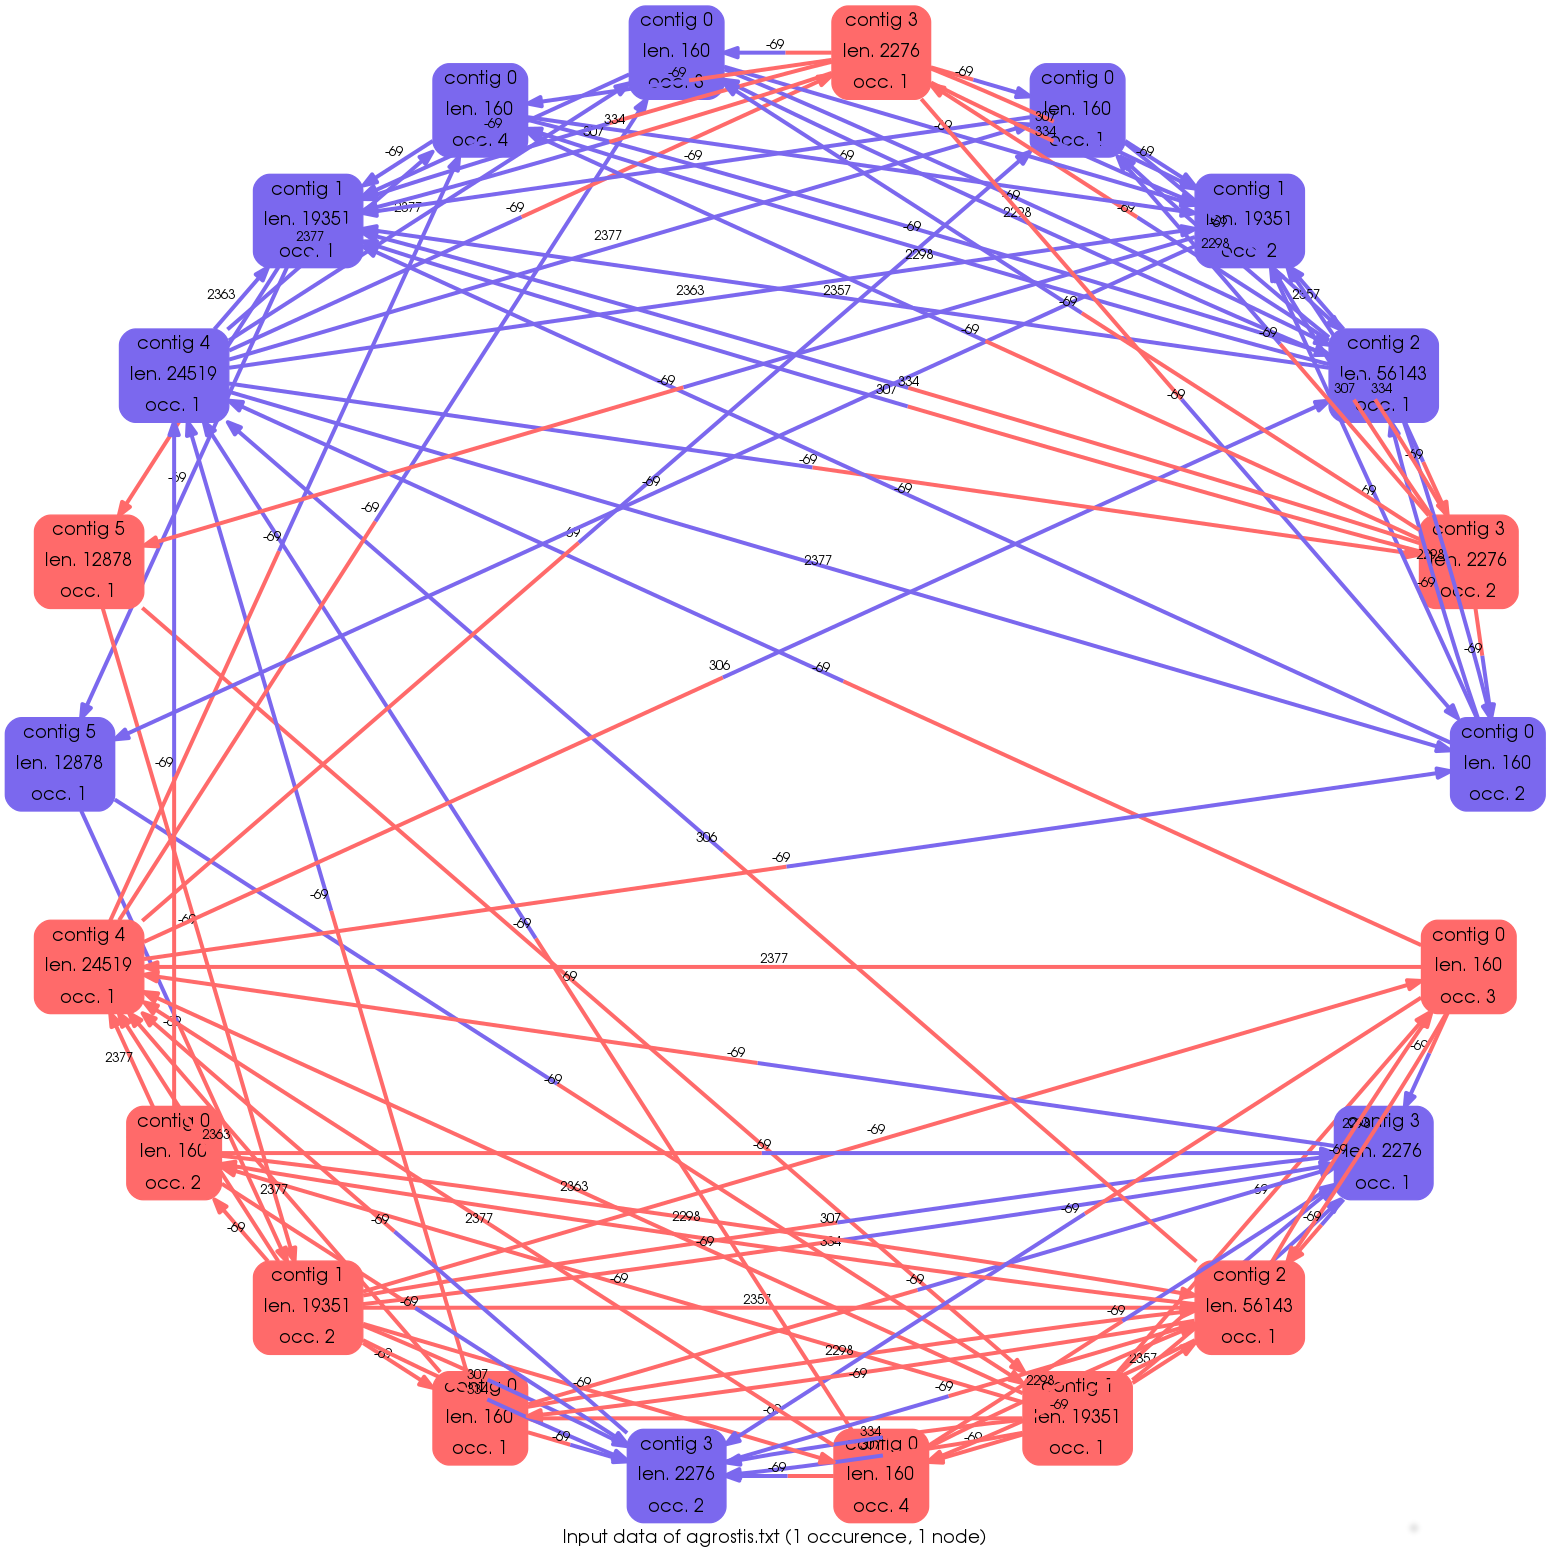
\includegraphics[scale=0.13]{agrostis_INPT_graph_model.png}
\end{minipage}
%
\begin{minipage}{0.25\textwidth}
\tiny
$\sum nodes = \sum cov. \times 2$ \\
\vspace*{0.2cm}
\begin{tabular}{ | c | c | c |}
  \hline  
unitig & len & cov \\\hline         
1 & 19351 & [2, 2]\\
0 & 160   & [2, 4]\\
3 & 2276  & [2, 2]\\
2 & 56143 & [1, 1]\\
5 & 12878 & [1, 1]\\
4 & 24519 & [1, 1]\\
  \hline  
\end{tabular}
\end{minipage}

\end{frame}

\subsection{Expected solution}\label{exp}
\begin{frame}
\frametitle{\textsc{\nameref{exp}}}
{\textit{Agrostis stolonifera} chpl. genome expected solution} \\
\begin{minipage}{0.65\textwidth}
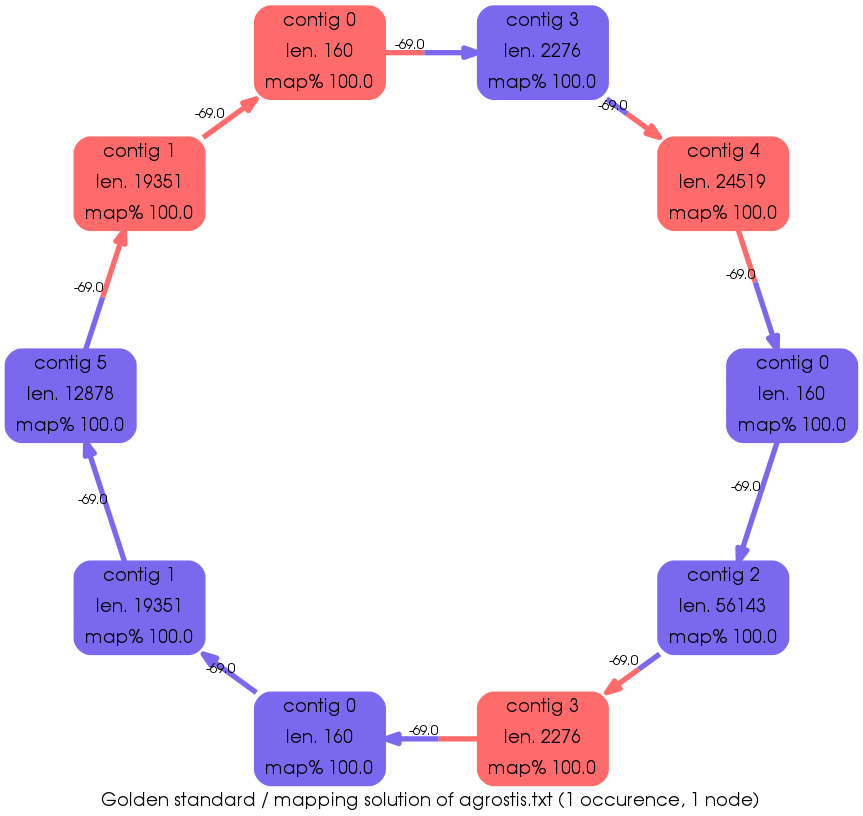
\includegraphics[scale=0.2]{agrostis_GOLD.png}
\end{minipage}
%
\begin{minipage}{0.3\textwidth}
\tiny
\textsc{\textcolor{magenta}{$\to$use unitigs the right number of times in the correct orientation \\ $\to $order unitigs to obtain an uninterrupted circular path}} \\
\vspace*{0.7cm}

\begin{tabular}{ | c | c | c |}
  \hline  
unitig & orient. & occ. \\\hline         
1 & reverse & 1\\
1 & forward & 1\\
3 & reverse & 1\\
3 & forward & 1\\
0 & reverse & 1\\
0 & forward & 2\\
  \hline  
\end{tabular}
\end{minipage}

\end{frame}


\subsection{Scaffolding solutions}\label{scafsols}
\begin{frame}
\frametitle{\textsc{\nameref{scafsols}}}
{\textit{Agrostis stolonifera} chpl. genome scaffolding solutions} \\
\vspace*{0.5cm}
\footnotesize \textsc{\textcolor{magenta}{Unitigs forming the inverted repeated sequence of the chloroplastic genome are duplicated. }}
\begin{center}
\resizebox{9cm}{!}{
\begin{tikzpicture}
\node (wpm1) at (0,0) {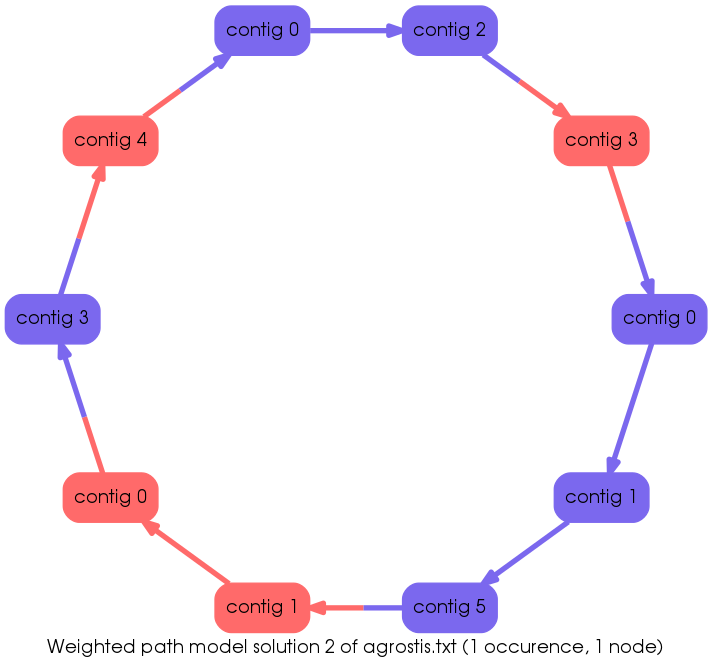
\includegraphics[scale=0.25]{wpm_agrostis_sol1}};
\node (wmp2) at (8,0) {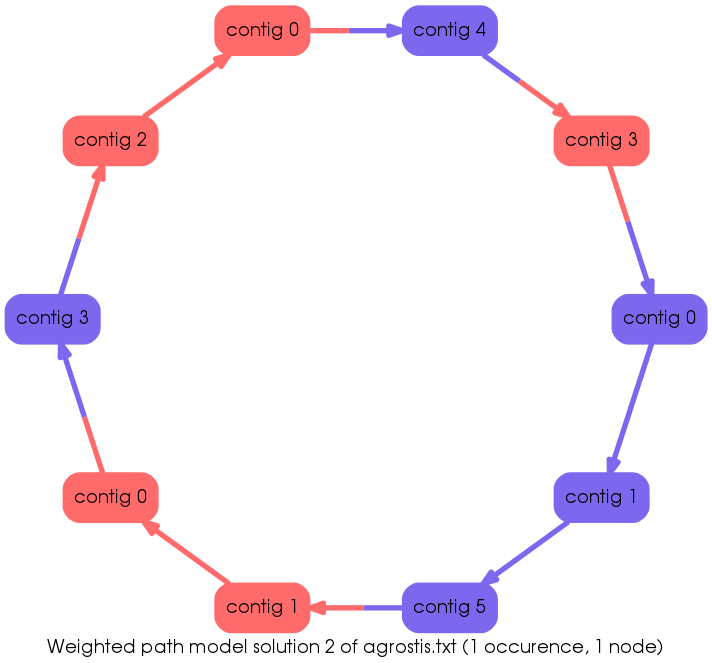
\includegraphics[scale=0.25]{wpm_agrosti_sol2}};
\node (gold) at (4,4.5) {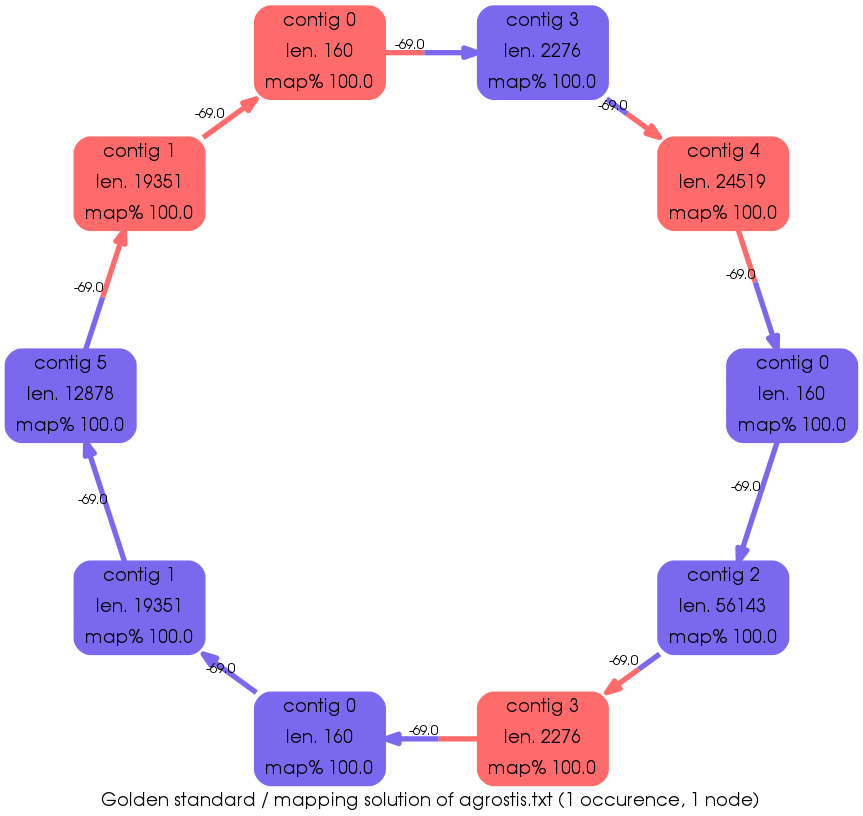
\includegraphics[scale=0.1]{agrostis_GOLD}};

\draw [blue!30,ultra thick,domain=-30:40] plot ({3.3*cos(\x)}, {3.3*sin(\x)});
\draw [blue!30,ultra thick,domain=175:235] plot ({3.3*cos(\x)}, {3.3*sin(\x)});
\draw [blue!30,ultra thick,domain=240:255] plot ({3.3*cos(\x)}, {3.3*sin(\x)});
\begin{scope}[shift={(8,0)}]
\draw [blue!30,ultra thick,domain=-30:40] plot ({3.3*cos(\x)}, {3.3*sin(\x)});
\draw [blue!30,ultra thick,domain=175:235] plot ({3.3*cos(\x)}, {3.3*sin(\x)});
\draw [blue!30,ultra thick,domain=240:255] plot ({3.3*cos(\x)}, {3.3*sin(\x)});
\end{scope}

\begin{scope}[shift={(4,4.5)}]
\draw [blue!30,ultra thick,domain=70:150] plot ({1.8*cos(\x)}, {1.8*sin(\x)});
\draw [blue!30,ultra thick,domain=210:290] plot ({1.8*cos(\x)}, {1.8*sin(\x)});

\end{scope}

\end{tikzpicture}
}
\end{center}

\end{frame}



\section{Benchmarking workflow for the GST}\label{bench}
\begin{frame}
\frametitle{\textsc{\nameref{bench}}}
\footnotesize \textsc{\textcolor{magenta}{Solutions found with the Genscale tools are benchmarked against the SSPACE published scaffolder.}}
\begin{center}
\resizebox{10cm}{!}{
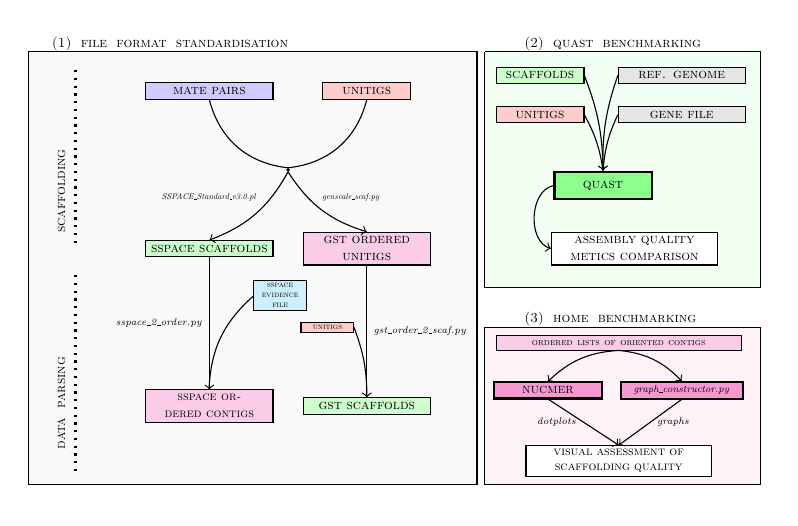
\begin{tikzpicture}
\node[text width=5cm,align=left] (filetit) [draw=none] at (0.5,0.6) {\textsc{\tiny (1) file format standardisation}};
\draw[fill=gray!5] (-2.3,0.5) -- (3.4,0.5) -- (3.4,-5) -- (-2.3,-5) -- (-2.3,0.5);
\node[text width=3cm,align=center] (mp) [draw, fill=blue!20, scale=0.5] at (0,0) {\textsc{mate pairs}};
\node[text width=2cm,align=center] (unitigs) [draw, fill=red!20, scale=0.5] at (2,0) {\textsc{unitigs}};

\node (arrowbase) [draw=none, shape=circle, fill=black, scale=0.15] at (1,-1) {};

\node[text width=3cm,align=center] (scaf) [draw, fill=green!20, scale=0.5] at (0,-2) {\textsc{sspace scaffolds}};
\node[text width=3cm,align=center] (list) [draw, fill=magenta!20, scale=0.5] at (2,-2) {\textsc{gst ordered unitigs}};

\draw (unitigs.south) to [bend left=35] (arrowbase.north);
\draw (mp.south) to [bend left=-35] (arrowbase.north);

\draw[->] (arrowbase.south) to [bend left=20] (scaf.north);
\draw[->] (arrowbase.south) to [bend right=20] (list.north);

\node[scale=0.3] (scafsspace) at (0, -1.35) {\textit{SSPACE\_Standard\_v3.0.pl}} ;
\node[scale=0.3] (scafgst) at (1.8, -1.35) {\textit{genscale\_scaf.py}} ;

\node[text width=3cm,align=center] (list2) [draw, fill=magenta!20, scale=0.5] at (0,-4) {\textsc{\small sspace ordered contigs}};
\node[text width=3cm,align=center] (scaf2) [draw, fill=green!20, scale=0.5] at (2,-4) {\textsc{gst scaffolds}};

\draw [->] (scaf.south) -- node[scale=0.7, left] {\tiny \textit{sspace\_2\_order.py}} (list2.north);
\draw [->] (list.south) -- node[scale=0.7, right] {\tiny \textit{gst\_order\_2\_scaf.py}} (scaf2.north);

\node[text width=2cm,align=center] (evidence) [draw, fill=cyan!20, scale=0.3] at (0.9,-2.6) {\textsc{sspace evidence file}};
\draw (evidence.west) to [bend right=23] (list2);

\node[text width=2cm,align=center] (unitigsbis) [draw, fill=red!20, scale=0.3] at (1.5,-3) {\textsc{unitigs}};
\draw (unitigsbis.east) to [bend left=10] (scaf2);

%somearrows
\node (A) [draw=none, shape=circle] at (-1.7,0.5) {};
\node (B) [draw=none, shape=circle] at (-1.7,-2.1) {};
\node (C) [draw=none, shape=circle] at (-1.7,-5) {};

\draw[sloped, anchor=center, above, text width=2.0cm, thick, dotted] (B) -- node{\tiny \textsc{scaffolding}} (A);


\draw[sloped, anchor=center, above, text width=2.0cm,thick, dotted] (C) -- node{\tiny \textsc{data parsing}}(B);

%benchmarking titles
\node[text width=3cm,align=left] (quasttit) [draw=none] at (5.5,0.6) {\textsc{\tiny (2) quast benchmarking}};
\node[text width=3cm,align=left] (hometit) [draw=none] at (5.5,-2.9) {\textsc{\tiny (3) home benchmarking}};
\draw[fill=green!5] (3.5,0.5) -- (7,0.5) -- (7,-2.5) -- (3.5,-2.5) -- (3.5,0.5);
\draw[fill=magenta!5] (3.5,-3) -- (7,-3) -- (7,-5) -- (3.5,-5) -- (3.5,-3);
%benchmarking quast guts
\node[text width=2cm,align=center] (scafs) [draw, fill=green!20, scale=0.5] at (4.2,0.2) {\textsc{scaffolds}};
\node[text width=2cm,align=center] (unitigs) [draw, fill=red!20, scale=0.5] at (4.2,-0.3) {\textsc{unitigs}};
\node[text width=3cm,align=center] (refgenome) [draw, fill=gray!20, scale=0.5] at (6,0.2) {\textsc{ref. genome}};
\node[text width=3cm,align=center] (gfile) [draw, fill=gray!20, scale=0.5] at (6,-0.3) {\textsc{gene file}};
\node[text width=1cm, align=center] (quastbam) [draw, thick, fill=green!45] at (5,-1.2) {\textsc{\tiny quast}};
\draw[thin, ->] (scafs.east) to [bend left=10] (quastbam.north);
\draw[thin, ->] (refgenome.west) to [bend left=-10] (quastbam.north);
\draw[thin] (unitigs.east) to [bend left=10] (quastbam.north);
\draw[thin] (gfile.west) to [bend left=-10] (quastbam.north);
\node[text width=4cm, align=center] (metrics) [draw, fill=white, scale=0.5] at (5.4,-2) {\textsc{assembly quality metics comparison}};
\draw[thin, ->] (quastbam.west) to [bend left=-75] (metrics.west);
%benchmarking home guts
\node[text width=6cm,align=center] (orders) [draw, fill=magenta!20, scale=0.5] at (5.2,-3.2) {\textsc{\scriptsize ordered lists of oriented contigs}};
\node[text width=2.5cm,align=center] (mummer) [draw, thick, fill=magenta!40, scale=0.5] at (4.3,-3.8) {\textsc{nucmer}};
\node[text width=3.2cm,align=center] (constructor) [draw, thick, fill=magenta!40, scale=0.45] at (6,-3.8) {\textit{\footnotesize graph\_constructor.py}};

\draw[thin, ->] (orders.south) to [bend left=-20] (mummer.north);
\draw[thin, ->] (orders.south) to [bend left=20] (constructor.north);

\node[text width=5cm,align=center] (viz) [draw, fill=white, scale=0.45] at (5.2,-4.7) {\textsc{visual assessment of scaffolding quality}};

\draw [->] (mummer.south) -- node[scale=0.7, left] {\tiny \textit{dotplots}} (viz.north);
\draw [->] (constructor.south) -- node[scale=0.7, right] {\tiny \textit{graphs}} (viz.north);
\end{tikzpicture}
}
\end{center}
\end{frame}

\section{Results}\label{15}
\begin{frame}
\frametitle{\textsc{\nameref{15}}}
Using the benchmark workflow the following conclusions were drawn: 
\begin{itemize}
\item Genomes with big repeated regions are solved a lot better with GSTs than with SSPACE
\item Small repeats are very challenging to scaffold because too many conflicting links exist and GST can not take a decision or is too slow
\item The GST models processing the link sequence length information perform worse than those focusing only on ordering and orientating
\end{itemize}
\end{frame}

\subsection{Large repeats}\label{largerepeats}
\begin{frame}
\frametitle{\textsc{\nameref{largerepeats} - chloroplastic genomes}}
\begin{center}
\footnotesize \textsc{\textcolor{magenta}{Excellent results are obtained for data sets with large repeats and a small number of unitigs.}} \\
\vspace*{0.2cm}
\resizebox{8cm}{!}{
\begin{tikzpicture}
\node (wpm1) at (0,0) {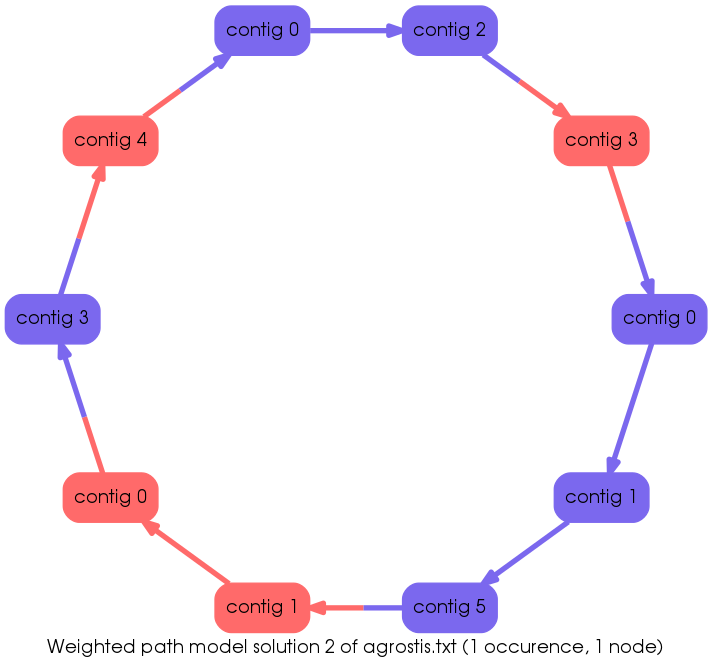
\includegraphics[scale=0.25]{wpm_agrostis_sol1}};
\node (wmp2) at (8,0) {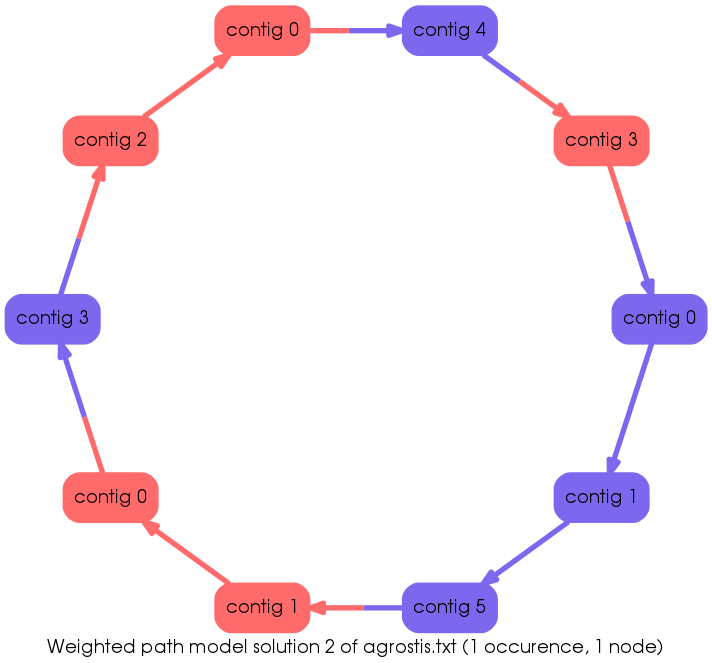
\includegraphics[scale=0.25]{wpm_agrosti_sol2}};
\node (sspace) at (9,7) {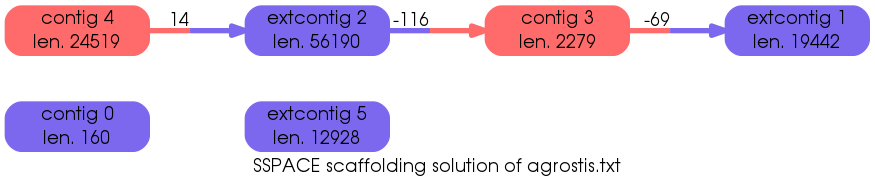
\includegraphics[scale=0.25]{sspace_scaffolds_agrostis}};
\node (gold) at (0,7) {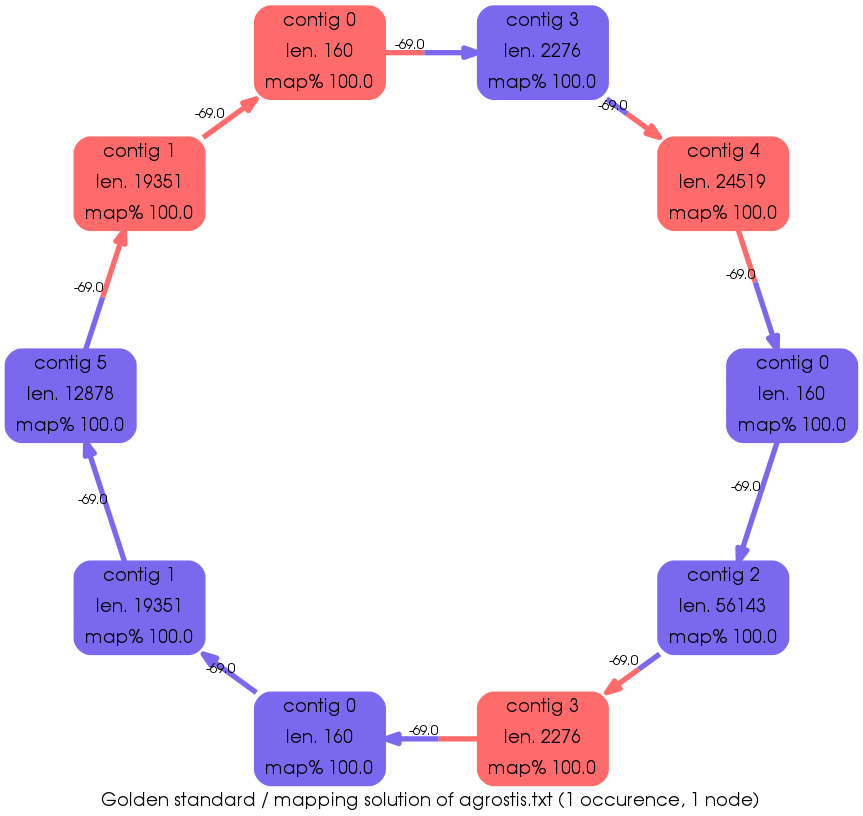
\includegraphics[scale=0.25]{agrostis_GOLD}};

\draw [blue!30,ultra thick,domain=-30:40] plot ({3.3*cos(\x)}, {3.3*sin(\x)});
\draw [blue!30,ultra thick,domain=175:235] plot ({3.3*cos(\x)}, {3.3*sin(\x)});
\draw [blue!30,ultra thick,domain=240:255] plot ({3.3*cos(\x)}, {3.3*sin(\x)});
\begin{scope}[shift={(8,0)}]
\draw [blue!30,ultra thick,domain=-30:40] plot ({3.3*cos(\x)}, {3.3*sin(\x)});
\draw [blue!30,ultra thick,domain=175:235] plot ({3.3*cos(\x)}, {3.3*sin(\x)});
\draw [blue!30,ultra thick,domain=240:255] plot ({3.3*cos(\x)}, {3.3*sin(\x)});
\end{scope}
\begin{scope}[shift={(0,7.1)}]
\draw [blue!30,ultra thick,domain=70:150] plot ({3.9*cos(\x)}, {3.9*sin(\x)});
\draw [blue!30,ultra thick,domain=210:245] plot ({3.9*cos(\x)}, {3.9*sin(\x)});
\draw [blue!30,ultra thick,domain=250:290] plot ({3.9*cos(\x)}, {3.9*sin(\x)});
\end{scope}
\begin{scope}[shift={(11,7.5)}]
\draw [blue!30,ultra thick,domain=0:360] plot ({2*cos(\x)}, {1*sin(\x)});
\end{scope}
\begin{scope}[shift={(5.9,6.7)}]
\draw [blue!30,ultra thick,domain=0:360] plot ({1*cos(\x)}, {0.5*sin(\x)});
\end{scope}
\end{tikzpicture}
}
\end{center}

\end{frame}

\subsection{Short repeats}\label{shortrepeats}
\begin{frame}
\frametitle{\textsc{\nameref{shortrepeats} - bacterial genomes}}
\scriptsize \textsc{\textcolor{magenta}{Small repeats are problematic starting from the unitig building step.} The Wolbachia Endosymbiont organism possesses 444 unitigs and only 138 are longer than 1000 base pairs.} \\
\vspace*{0.2cm}
\begin{center}
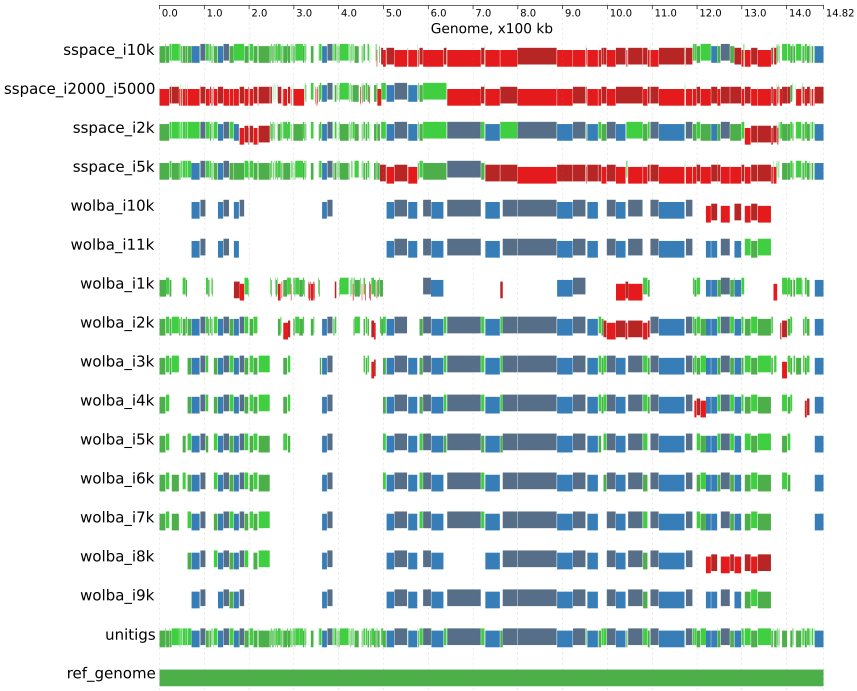
\includegraphics[scale=0.3]{alignment_woinserts.png}
\end{center}

\end{frame}

\section{Perspectives}\label{17}
\begin{frame}
\frametitle{\textsc{\nameref{17}}}
\begin{center}
\textsc{\textcolor{magenta}{Develop - Test - Benchmark}}
\end{center}
\begin{itemize}
\item Find strategies which solve more challenging data \\ $\to$ flow model in development
\item Benchmark against other tools trying to solve repeated regions
\item Test the GST with real data
\item Test the GST with other genome sequencing data types
\end{itemize}
\end{frame}
\section*{}
\begin{frame}
\frametitle{\textsc{Thank you for you attention}}
\begin{center}
\textsc{Scaffolding: safety comes first} \\
\vspace*{0.5cm}

\includegraphics[scale=1]{joke.jpg}
\end{center}
\end{frame}
%----------------------------------------------------------------------------------------

\end{document} 